% \documentclass[11pt,reqno,draft]{amsart}
\documentclass[11pt,reqno]{amsart}
%% Escrevendo em português:
\usepackage[brazil]{babel}
%\usepackage[T1]{fontenc}
\usepackage{lmodern}
%----------------------------

%----------------------------
%\documentclass[11pt,reqno]{amsart}
\usepackage[utf8x]{inputenc}
\usepackage{amsfonts}
\usepackage{amsmath,calc} %para usar ocm LPs
\usepackage{mathtools,amssymb} %para usar com LPs
\usepackage{amsthm}
\usepackage{subfigure}
\usepackage[toc,page]{appendix}
%\usepackage[subnum]{cases} %numerar
\usepackage{cases} %numerar

%rescaling letters
\usepackage{mathrsfs} %mathscr
\newcommand{\smallG}{\mbox{\larger[-1]$(G)$}}
\newcommand{\smallGf}{\mbox{\larger[-1]$(G-f)$}}
\newcommand{\smallGprime}{\mbox{\larger[-1]$(G')$}}
\newcommand{\smallGprimef}{\mbox{\larger[-1]$(G'-f)$}}
\newcommand{\smallGprimeG}{\mbox{\larger[-1]$(G',G)$}}
\newcommand{\smallW}{\mbox{\larger[-1]$(G[W])$}}
\newcommand{\smallWg}{\mbox{\larger[-1]$(G[W]-g)$}}
\newcommand{\smallWWbarf}{\mbox{\larger[-1]$(G[E(W) \cup E(\overline{W})+f])$}}
\newcommand{\smallWWbarfg}{\mbox{\larger[-1]$(G[E(W) \cup E(\overline{W})+f-g])$}}
\newcommand{\smallH}{\mbox{\larger[-1]$(H)$}}
\newcommand{\smallF}{\mbox{\larger[-1]$(G[F])$}}
\newcommand{\spanPath}{\mathcal{P}}
\newcommand{\spanBridge}{\mathcal{B}}
\newcommand{\Pathuv}{\spanPath_{u,v}^{t}}
\newcommand{\Pathpq}{\spanPath_{p,q}^{t}}
\newcommand{\Path}{\spanPath^{t}}
\newcommand{\PathuvF}{\Pathuv\smallF}
\newcommand{\PathuvGprime}{\Pathuv\smallGprime}
\newcommand{\PathuvGprimef}{\Pathuv\smallGprimef}
\newcommand{\PathuvGf}{\Pathuv\smallGf}
\newcommand{\PathpqW}{\Pathpq\smallW}
\newcommand{\PathpqWg}{\Pathpq\smallWg}
\newcommand{\PathpqWWbarf}{\Pathpq\smallWWbarf}
\newcommand{\PathpqWWbarfg}{\Pathpq\smallWWbarfg}
\newcommand{\BridgeuvPrime}{\spanBridge_{u',v'}^{t}}
\newcommand{\Bridgeuv}{\spanBridge_{u,v}^{t}}
\newcommand{\Bridge}{\spanBridge^{t}}
\newcommand{\smallQBridge}{\mbox{\larger[-1]$(Q \cup \Bridge)$}}
\newcommand{\PathuvQBridge}{\Pathuv\smallQBridge}
\newcommand{\BridgeuvGprime}{\Bridgeuv\smallGprime}
\newcommand{\BridgeuvPrimeGf}{\spanBridge_{u',v'}^{t}\smallGf}
\newcommand{\BridgeuvGf}{\Bridgeuv\smallGf}
\newcommand{\BridgeGf}{\Bridge\smallGf}
\newcommand{\BridgeuvGprimeG}{\Bridgeuv\smallGprimeG}
\newcommand{\BridgeTwo}{\spanBridge_{2}^{t}}
\newcommand{\BridgeGprime}{\Bridge\smallGprime}
\newcommand{\BridgeTwoGprime}{\BridgeTwo\smallGprime}
\newcommand{\BridgeTwoGf}{\BridgeTwo\smallGf}


%-----largura do texto
 \setlength{\textwidth}{33pc}
 \setlength{\textheight}{50pc}
 \setlength{\oddsidemargin}{2.5cm}
 \setlength{\evensidemargin}{2.5cm}
 \setlength{\hoffset}{-0.5in}

 \setlength{\voffset}{-0.7in}
%--------------

\usepackage{siunitx}

%LP formulation
\usepackage{lpform} %LPs
\renewcommand{\lpforall}[1]{&& \forall #1}

\newcommand{\dist}{{\rm dist}}
\newcommand{\maxdist}{{\rm maxDist}}

%reset equation number whenever section and subsection is stepped
\usepackage{chngcntr}
\counterwithin*{equation}{section}
\counterwithin*{equation}{subsection}

%meus ambientes
\newtheorem{definicao}{Definição}
\newtheorem{notacao}{Notação}
%\newtheorem{teorema}{Teorema}[section]
\newtheorem{teorema}{Teorema}
\newtheorem{proposition}{Proposition}
\newtheorem{afirmacao}{Afirmação}[teorema]
%\newtheorem{lema}{Lema}[section]
\newtheorem{lema}{Lemma}
\newtheorem{observacao}{Observação}
%\newtheorem{proposicao}{Proposição}[section]
\newtheorem{proposicao}{Proposição}
%\newtheorem{corolario}{Corolário}[section]
\newtheorem{corolario}{Corolário}
\newtheorem{conjectura}{Conjectura}
\newtheorem{problema}{Problema}
\newtheorem{exemplo}{Exemplo}

%comandos para novas letras/exppressões
\newcommand{\incid}{\mathcal{X}}
\newcommand{\incidY}{\mathcal{Y}}
\newcommand{\maxstretchfactor}{\mathcal{T}}
\newcommand{\espacoX}{\mathbb{R}^{|E(G)|}}
\newcommand{\espacoY}{\mathbb{R}^{|E(G)| \times |E(G)|}}
\newcommand{\PGtrestricoes}{(PL)}
\newcommand{\facetF}{\mathcal{F}}

\title{MMST}
\author{Hugo Braga}
\date{2015}

\begin{document}

\maketitle

\section{Introdução}
Neste texto, a menos de menção em contrário, os grafos considerados
são não-orientados, simples e conexos.  Dado um grafo $G=(V,E)$, 
uma função custo $w: E \to \mathbb{R}^+$ e um
natural $t \ge 1$, chamado de \emph{fator de dilatação}, um
\emph{$t$-spanner} é um subgrafo gerador $H$ de $G$ tal que:
\begin{equation}
%\label{eq:spanner}
\dist_{H}(u,v) \le t \cdot \dist_{G}(u,v), \quad \forall\;u,v \in V, 
\label{eq:def_spanner}
\end{equation}

\noindent onde $\dist_{G}(u,v)$ denota a distância entre $u$ e $v \in V$. 
A distância entre $u$ e $v$ em $G$ é calculada através do 
somatório do custo (definido pela 
função $w$) das arestas de um caminho de custo mínimo entre $u$ e $v$ em $G$. 
Seja $(\incid^{H})_{e \in E(G)}$ o vetor de incidência de $H$. 
Quando $H$ é uma árvore dizemos que $H$ é uma \emph{árvore $t$-spanner}. 
Para $u,v \in V(H)$, seja $H_{u,v}$ o caminho entre $u$ e $v$ na árvore  $H$.
Além disso, para um grafo $G$, considere $V(G)$ o conjunto 
dos vértices de $G$ e $E(G)$ o conjunto das arestas de $G$. 
Um caminho $P_{u,v} \subseteq G$ é um caminho $t$-spanner com 
relação a $G$ entre os vértices $u,v \in V(G)$ se 
$dist_{P_{u,v}}(u,v) \le t \cdot dist_{G}(u,v)$. 
% Ademais, 
% considere um $(u,v,t,G',G)$-caminho como sendo um caminho $t$-spanner com 
% relação a $G$ entre 
% os vértices $u,v \in V(G)$, e que está contido em $G' \subseteq G$. Quando 
% não for importante mencionar o subgrafo onde o caminho $t$-spanner está contido,
%  nos referiremos apenas como um $(u,v,t,G)$-caminho.

Cai e Corneil \cite{CaiC1995} 
mostraram que várias definições de t-spanner são equivalentes. 
Seja $Q$ um subgrafo gerador conexo de $G$.
Dentre as definições que são equivalentes com (\ref{eq:def_spanner}), estão:

\begin{equation}
\dist_{Q}(u,v) \le t \cdot \dist_{G}(u,v), \quad \forall\;uv \in E(G).
\label{eq:def2_spanner}
\end{equation}

A prova de que (\ref{eq:def_spanner}) implica em (\ref{eq:def2_spanner}) 
é direta. 
Vamos provar que (\ref{eq:def2_spanner}) implica em (\ref{eq:def_spanner}). 

\begin{observacao}
\label{obs:relate_spanner_definitions}
Seja $Q$ um subgrafo gerador conexo de $G$. Então
\begin{equation*}
\begin{split}
\dist_{Q}(u,v) \le t \cdot \dist_{G}(u,v), \forall\;uv \in E(G) \implies \\
\dist_{Q}(u,v) \le t \cdot \dist_{G}(u,v), \forall\;u,v \in V(G).
\end{split}
\end{equation*}
\begin{proof}
Seja $u,v \in V(G)$. Se $uv \in E(G)$, por hipótese, segue a conclusão. 
Vamos assumir que $uv \notin E(G)$. Seja 
$P = (u = u_0, u_1, ..., u_{l-1}, u_l = v)$ um caminho de custo mínimo entre 
$u$ e $v$ em $G$. Por hipótese, para cada \\
\mbox{$u_{i-1}u_i \in E(P), \dist_{Q}(u_{i-1},u_i) \le t \cdot \dist_{G}(u_{i-1},u_i)$}.
 Então: 
\begin{align*}
\dist_{Q}(u,v) &= \sum_{i = 1}^{l} dist_{Q}(u_{i-1},u_i)\\ 
&\le \sum_{i = 1}^{l}t \cdot \dist_{G}(u_{i-1},u_i)\\
&= t \cdot \sum_{i = 1}^{l} \dist_{G}(u_{i-1},u_i)\\
&= t \cdot \dist_{G}(u,v),
\end{align*}
onde a primeira e última igualdade seguem do fato de que o custo de um 
caminho de custo mínimo é igual ao somatório do custo das arestas que compoem o 
caminho.
\end{proof}
\end{observacao}

Uma versão de otimização para o problema de árvore \hbox{$t$-spanner}
corresponde em minimizar o fator de dilatação. Formalmente, o problema
é definido como: dado um grafo $G=(V,E)$ e uma 
função custo $w: E \to \mathbb{R}^+$, o \emph{problema de árvore spanner mínima}
(\emph{Minimum Max-Stretch Spanning Tree} - MMST) tem por objetivo
encontrar o menor~$t$ (natural) tal que $G$ admite uma árvore
$t$-spanner. 

\section{Poliedro dos Grafos t-spanner}
Para um grafo $G$ e um natural $t \ge 1$, o poliedro do problema de grafos (não 
necessariamente árvores) $t$-spanner é definido como 

% O problema do MMST pode ser visto da seguinte forma: dado um grafo $G$, o 
% objetivo é encontrar um subgrafo $H$ t-spanner de $G$ que minimiza o número de 
% arestas e minimiza o fator de dilatação $t$. Observe que o conjunto de soluções 
% viáveis corresponde ao conjunto de todos os subgrafos $H$ (não necessariamente 
% árvore) t-spanner de $G$. Como estamos assumindo que os grafos 
% de entrada são conexos, para que um grafo $H$ seja solução viável, é necessário 
% que $H$ seja conexo. Como o objetivo é minimizar o número de arestas, e o grafo 
% conexo com menor número de arestas é uma árvore, segue que a solução é uma 
% solução do MMST. 
% Desta forma, o seguinte poliedro é válido para o MMST: 

\begin{equation*}
\begin{split}
P_{span}(G,t) \leftarrow \text{conv}\{\incid^{F} \in \espacoX\; |\; \text{$G[F]$ é um grafo $t$-spanner\}}. 
\end{split}
\end{equation*}
Observe que $\forall t" \ge t', P_{span}(G,t') \subseteq P_{span}(G,t")$. 

Seja $\maxdist_G(u,v)$ o custo de um caminho de custo máximo entre $u,v \in V(G)$. 
Seja $\maxstretchfactor' = max_{u,v \in V(G)}\frac{\maxdist_G(u,v)}{\dist_G(u,v)}$. 
Seja $\maxstretchfactor = \lceil \maxstretchfactor' \rceil$.
Então, $\forall t" \ge \maxstretchfactor, P_{span}(G,\maxstretchfactor) = P_{span}(G,t")$.
% É fácil observar que 

% Seja $e=uv \in E(G)$. Seja $\incidY(e)^{S} \in \{0,1\}^{E}$ 
% o vetor de incidência tal que $\forall f \in E(G), \incidY(e)_{f} = 1$ se $\exists (u,v,t,G[S],G)$-caminho passando por $f$$P$. 
% %tal que $Y(e,f) = 1, \forall f \in E(P)$. 
% Para $t \ge 1$, seja $HC \in \{0,1\}^{E}$ o vetor de incidência tal que $HC_{e}^{S} = 1$ se 
% $\forall u,v \in V(G) \not \exists (u,v,t,G[S],G)$-caminho passando por $e$. 
% Então, $P_{span}(G,t)$ pode ser escrito da 
% seguinte forma:

% \begin{equation*}
% \begin{split}
% P_{span}(G,t) \leftarrow \text{conv}\{(\incidY(e_1), .., \incidY(e_m))^{S}\; |\; \text{$G[S]$ é um grafo $t$-spanner e }\\ 
% \text{$\forall f \in S\; \exists u,v \in V(G)\; \exists (u,v,t,G)$-caminho passando por $f$}\}.
% \end{split}
% \end{equation*}
% Note que 
% $\{f \in E(G): \incid_{f}^{S} = 1\} = \{f \in E(G): \exists_{e \in E(G)} \incidY(e)_{f}^{S} = 1\text{ ou }HC_{f}^{S} = 1\}$.

\subsection{Solução do MMST}
\label{sec:poliedro_sol_mmst}

%Seja $M$ um número bem grande. 
Uma solução $H$ para o MMST pode ser expressa da seguinte forma: 

\begin{equation*}
\begin{split}
H = arg\_min_{t}\{F \subseteq E(G)\ |\; \exists \incid^{F} \in P_{span}(G,t)\text{ tal que }\\
G[F]\text{ é uma árvore geradora de }G, 1 \le t \le \maxstretchfactor\}.
\end{split}
\end{equation*}

Em outras palavras, eu quero descobrir o menor poliedro $P_{span}(G,t)$ (literalmente, 
pois $P_{span}(G,t') \subseteq P_{span}(G,t"), \forall t" \ge t'$) o qual possui 
como solução uma árvore.

% Note que a adição do $M$ na função a ser minimizada é necessário para que a 
% solução seja uma árvore. Por exemplo, considere o grafo triângulo como grafo 
% de entrada, cujo custo das arestas é uniforme e com valor $1$. 
% Seja $z = t + |S|)$. 
% Uma solução ótima $S$ para o MMST 
% é um subgrafo com duas arestas, cujo valor de $z$ 
% associado é $2 + 2 = 4$. Mas, observe que a solução $S'$ correspondendo ao 
% próprio grafo triângulo também é uma solução viável de $P_{span}(G,1)$, cujo 
% valor de $z$ associado é $1 + 3 = 4$. Neste caso, $S'$ também seria considerada 
% uma solução ótima, mas não seria uma solução para o MMST.

\subsection{Dimensão do poliedro}
Seja $G'$ um $t$-spanner de $G$. 
Seja $\PathuvGprime$ a coleção de caminhos $t$-spanner 
com relação a $G$ entre os vértices $u,v \in V(G)$, e que estão contidos em 
$G'$.

Uma aresta $f \in E(G')$ é chamada de 
\emph{ponte $t$-spanner} de $G'$ se e somente se $G'-f$ não é $t$-spanner 
de $G$. Mais especificadamente, $f \in E(G')$ é ponte $t$-spanner de $G'$ para 
$u,v \in V(G)$ 
se e somente se $\PathuvGprimef = \emptyset$. 
Seja $\BridgeuvGprime$ o conjunto destas pontes. 
Seja \mbox{$\BridgeGprime = \bigcup_{u,v \in V(G)} \BridgeuvGprime$}. 
Seja $\BridgeTwoGprime \subseteq 2^{V(G)}$ tal que 
$\BridgeuvGprime \neq \emptyset, \forall (u,v) \in \BridgeTwoGprime$. 
Quando $G' = G$, 
utilizaremos as notações $\Path, \Bridgeuv, \Bridge, \BridgeTwo$. 

No lema a seguir, provamos a dimensão do poliedro.

\begin{lema}
$dim(P_{span}(G,t)) = |E(G)| - |\Bridge|$.
\begin{proof}
Seja $f \in \Bridge$. Então, para cada $\incid^{F} \in P_{span}(G,t)$, segue que 
$f \in F$. Sendo assim, $P_{span}(G,t) \subseteq \{x(f) = 1\}$. Logo, 
$dim(P_{span}(G,t)) \le |E(G)| - |\Bridge|$.

Como $G$ é $t$-spanner, $\incid^{E(G)} \in P_{span}(G,t)$ e 
$\incid^{E(G)-f} \in P_{span}(G,t), \forall f \in E(G) \setminus \Bridge$. Então 
$dim(P_{span}(G,t)) \ge |E(G)| - |\Bridge|$, concluindo a prova.
\end{proof}
\end{lema}

Vamos agora mostrar que $P_{span}(G,t)$ não tem dimensão plena. Antes disso, 
precisamos de um lema auxiliar.

\begin{lema}
\label{lem:ordem_pontes}
Para cada caminho em $\Pathuv$, as arestas de 
$\Bridgeuv$ aparecem na mesma ordem.

\begin{proof}
Seja $P = (u_0, u_1, ..., u_i, u_{i+1} = v_i, u_{i+2}, .., u_j, u_{j+1} = v_j, .., v)$ 
um caminho de custo mínimo entre $u$ e $v$ em $G$. Observe que $P \in \Pathuv$.  Seja $u_iv_i,u_jv_j \in \Bridgeuv$. Suponha (por absurdo) que 
existe um caminho $P' \in \Pathuv$ tal que $u_jv_j$ apareça antes de $u_iv_i$ em 
$P'$. Temos que considerar dois casos: 

\begin{itemize}
\item $u_j$ antecede $v_j$ em $P'$: podemos assumir que 
$\dist_{P}(u_j,v) > \dist_{P'}(u_j,v)$. Caso contrário, seja $P'(u,u_j)$ o 
subcaminho de $P'$ entre $u$ e $u_j$. De maneira semelhante, defina $P(u_j,v)$. 
Então a concatenação entre $P'(u,u_j)$ e $P(u_j,v)$ contém um caminho 
$P_{u,v} \in \Pathuv$ que não contém $u_iv_i$, contradizendo o fato de 
$u_iv_i \in \Bridgeuv$.
 
%$t$-spanner para $u,v$.

Como sabemos que $u_j \in V(P)$, a relação 
$\dist_{P'}(u_j,v) < \dist_{P}(u_j,v)$ contradiz o fato de $P$ ser um caminho 
de custo mínimo entre $u$ e $v$ em $G$, pois a concatenação de $P(u,u_j)$ com 
$P'(u_j,v)$ contém um caminho entre $u$ e $v$ cujo custo é menor do que o de $P$.

\item $v_j$ antecede $u_j$ em $P'$: a prova é semelhante ao caso anterior, 
substituindo $u_j$ por $v_j$ na argumentação.
\end{itemize}
\end{proof}
\end{lema}

% \begin{lema}
% \label{lem:no_bridges}
% Seja $u,v \in V(G)$ e seja $B_G(u,v,t) = \{u_1v_1, u_2v_2, ..., u_pv_p\}$. 
% Sem perda de 
% generalidade, para cada $(u,v,t,G)$-caminho, assuma que $u_iv_i \in B_G(u,v,t)$ 
% aparece antes de $u_jv_j$, para $j > i$ (lema \ref{lem:ordem_pontes}). 
% Vamos denominar $u$ de $v_0$ e $v$ de $u_{p+1}$. 
% Então, $\forall 0 < i \le p+1$, não existe $(v_{i-1},u_{i},t,G)$-ponte.
% \begin{proof}
% Suponha (por absurdo) que $\exists f \in E(G)$ tal que 
% $f \in B_G(v_{i-1},u_{i},t)$, $0 < i \le p+1$. Sem perda de generalidade, seja 
% $0 < i < p+1$.  
% Seja $P$ um $(u,v,t,G)$-caminho. 
% Como $u_iv_i$ é a $i$-ésima $(u,v,t,G)$-ponte, 
% seja 
% $P' \subseteq P$ o caminho entre $v_{i-1}$ e $u_i$ em $P$. Como 
% $f \in B_G(v_{i-1},u_{i},t)$, 
% então $f \in P'$ e, por consequência, $f$ é uma $(u,v,t,G)$-ponte. 
% Mas isto contradiz o fato de $u_iv_i$ ser a $i$-ésima $(u,v,t,G)$-ponte.
% \end{proof}
% \end{lema}

Sem perda de generalidade, vamos assumir que para 
$\Bridgeuv = \{u_1v_1, u_2v_2, .., u_pv_p\}$, 
onde $u_iv_i$ aparece antes de $u_{i+1}v_{i+1}$ em cada caminho em $\Pathuv$, 
para cada $u_iv_i,u_{i+1}v_{i+1} \in \Bridgeuv$ (lema \ref{lem:ordem_pontes}).
\begin{proposicao}
\label{prop:dimensao_nao_plena}
Seja $G' \leftarrow G \setminus \Bridge$. Então, 
para $Q \subseteq G'$, $Q \cup \Bridge$ contém um subgrafo $t$-spanner de $G$ 
se e somente se 
para cada $(u,v) \in \BridgeTwo$ 
e $\Bridgeuv = \{u_1v_1, u_2v_2, .., u_pv_p\}$, 

\begin{equation*}
\dist_{Q}(u,u_1) + \dist_{Q}(v_1,u_2) + ... + \dist_{Q}(v_p,v) \le t \cdot \dist_{G}(u,v) - \sum_{u_iv_i \in \Bridgeuv} c(u_iv_i).
\end{equation*}
\begin{proof}
Seja $Q_{x,y}$ um caminho de custo mínimo em $Q$ entre $x,y \in V(G)$. 

$(\Rightarrow)$ Seja $(u,v) \in \BridgeTwo$. 
Suponha (por absurdo) que a inequação acima 
não seja válida. 
Como $Q \cup \Bridge$ contém um subgrafo $t$-spanner 
e vale o lema \ref{lem:ordem_pontes}, então 

\begin{equation*} 
Q_{u,u_1} \cdot u_1v_1 \cdot Q_{v_1,u_2} \cdot u_2v_2 \cdot ... \cdot Q_{v_p,v}
\end{equation*}
é um caminho de custo mínimo entre $u$ e $v$ em $Q \cup \Bridge$, 
cujo custo é maior do que $t \cdot dist_{G}(u,v)$, contradizendo o fato de 
existir um caminho em $\PathuvQBridge$.

$(\Leftarrow)$
Seja $(u,v) \in 2^{V(G)} \setminus \BridgeTwo$. $G'$ possui um caminho em 
$\PathuvGprime$ pois $\Bridgeuv = \emptyset$. %$G$ não tem $(u,v,t,G)$-ponte. 
Seja $(u,v) \in \BridgeTwo$. 
Como G é conexo e a inequação da hipótese é válida, então 
$P = Q_{u,u_1} \cdot u_1v_1 \cdot Q_{v_1,u_2} \cdot u_2v_2 \cdot ... \cdot Q_{v_p,v}$ 
é um caminho entre $u$ e $v$ em $G$ tal que 
$dist_P(u,v) \le t \cdot dist_G(u,v)$, concluindo a prova de que 
$Q \cup \Bridge$ contém um subgrafo $t$-spanner de $G$.
\end{proof}
\end{proposicao}

Em decorrência da inequação apresentada na proposição 
\ref{prop:dimensao_nao_plena}, caso o grafo de entrada $G$ possua pontes 
$t$-spanner, não podemos dividir o problema em problemas menores sem as 
pontes $t$-spanner. Consequentemente, $P_{span}(G,t)$ não tem dimensão plena.

\section{Formulação para o Poliedro dos Grafos t-spanner}
Seja $\incid^{F} \in P_{span}(G,t)$. 
Considere a variável de decisão $x \in \espacoX$ com o seguinte 
significado: $x(e), e \in E(G)$, é igual a 1 se e somente se $e$ faz parte da 
solução $F$  e 0 caso contrário. Considere a variável de decisão 
$Y \in \espacoY$ com o seguinte significado: 
para $e = uv \in E(G)$, 
existe $P \in \PathuvF$ tal que $Y(e,f) = 1, \forall f \in E(P)$. 
%$Y(e,f) = 1$ se existe um $(u,v,t,G[S],G)$-caminho passando por $f$.
% existe um $(u,v,t,G[S],G)$-caminho $P$ tal que $Y(e,f) = 1, \forall f \in E(P)$. 
% Se $Y$ possui suporte 
% mínimo, então o lado oposto da implicação também vale. 

Para $e \in E(G)$, considere $\delta(W)$ como sendo o conjunto de arestas que tem 
exatamente um dos vértices de $e$ em $W$. Considere o seguinte poliedro: 
%tal que $e$ faz parte deste conjunto de arestas.

\begin{lpformulation}[\PGtrestricoes]
%\lpobj*{min}{t + M \cdot x(E)}
\lpeq[res_mmst:path]{Y(e,\delta(W)) \ge 1}{e \in E, \forall W \subset V, |W \cap e| = 1}
%\lpeq[res_mmst:tree]{x(E) = |V| - 1}{}
\lpeq[res_mmst:relate_vars]{Y(e,f) \le x(f)}{e,f \in E}
\lpeq[res_mmst:spanner]{\sum_{f \in E(G)}Y(e,f) w(f) \le 
t \cdot \dist_{G}(u,v)}{e=uv \in E}
%\lpeq[res_mmst:t]{t \ge 1}{}
\lpeq[res_mmst:int_x]{0 \le x(e) \le 1}{e \in E}
\lpeq[res_mmst:int_Y]{0 \le Y(e,f) \le 1}{e,f \in E}
%\lpeq[res_mmst:real_t]{t \in \mathbb{R}^+}{}
%\lplabel{lp:primal_mmst}
\end{lpformulation}
% onde $\delta(S)$ corresponde ao conjunto de arestas que tem exatamente 
% um dos vértices em $S$.

%\begin{equation}
$P(G,t) \leftarrow \{(x \in \espacoX, Y \in \espacoY)\; |\; (x,Y) \in \PGtrestricoes\}$.
%\end{equation}

Ao longo desta seção, iremos provar que o fecho inteiro da projeção de $P(G,t)$ em $x$ 
é igual ao poliedro $P_{span}(G,t)$.

\begin{afirmacao}
\label{afirm:sol_viavel_lp} 
Para cada $\incid^{F} \in P_{span}(G,t)$, existe uma solução viável 
%$Sol = 
$(x', Y') \in (P(G,t))_{I}$. Ademais, $Y'$ possui suporte 
mínimo.
% Ademais, $Y'$ possui suporte mínimo.
% Para uma árvore $t'$-spanner $T$ de um grafo $G$, existe 
% uma solução viável $Sol = (x', Y', t')$ de \ref{lp:primal_mmst}. 
% Ademais, $Y'$ possui suporte mínimo.
\begin{proof}
Para $e=uv \in E(G)$, seja $P_{u,v} \in \PathuvF$. 
%o caminho mínimo numerado entre $u$ e $v$ em $G[S]$.
Para cada $e = uv, f \in E(G)$, 
defina $x'$ e $Y'$ da seguinte forma: 

\begin{align*}
&x'(e) \leftarrow \incid^{F}_{e},\\
&Y'(e,f)\leftarrow
\begin{cases}
    1& \text{se $f \in E(P_{u,v}),$}\\
    0& \text{caso contrário.}
    %0& \text{se $f \in E(G) \setminus E(P_{u,v}).$}
\end{cases}
\end{align*}

Seja $e = uv \in E(G)$ e $f = xy \in F$ tal que $Y'(e,f) = 1$. Note que 
$f \in E(P_{u,v})$. Seja 
$P_{u,v} = \{u = u_0, u_1, ., u_i = x, u_{i+1} = y, ..,  u_{l-1}, u_l = v\}$. 
Caso $Y'(e,f) \leftarrow 0$, para $W = \{u_0, u_1, .., u_i\}$ e a aresta $f$, 
a restrição \ref{res_mmst:path} é violada, 
pois $F(e) = \{g \in E: Y'(e,g) = 1 \text{ ou } g = f\}$ induz um caminho. 
Segue que $Y'$ tem suporte mínimo.
\end{proof}
\end{afirmacao}

Seja %$Sol = 
$(x',Y') \in (P(G,t))_{I}$ %uma solução ótima de \ref{lp:primal_mmst} 
tal que $Y'$ tem suporte mínimo. 
Para $e \in E(G)$, seja $F(e) = \{f \in E(G): Y'(e,f) = 1\}$. 
Seja $G' = G[\bigcup_{e \in E(G)}F(e)]$. 
Seja $E_{x} = \{e \in E(G): x'(e) = 1\}$. Seja $H = G[E_{x}]$.

A restrição \ref{res_mmst:path}
%é oriunda do trabalho de Goemans e Williamson \cite{GoemansW1995} e 
serve para garantir que $G'$ seja um subgrafo gerador conexo de $G$. A 
seguir, provaremos tal propriedade.

\begin{proposicao}
\label{prop:Yuv_caminho}
Para cada $e = uv \in E(G)$, existe um caminho entre $u$ e $v$ em 
$G[F(e)]$.
\begin{proof}
Seja $e = uv \in E(G)$. Suponha (por absurdo) que não existe um 
caminho entre $u$ e $v$ em $G[F(e)]$. Então $u$ e $v$ estão 
em componentes distintas em $G[F(e)]$. Seja $G_u$ o grafo induzido pelos 
vértices do componente de $G[F(e)]$ que contém $u$. Seja $W = V(G_u)$. Mas 
então a restrição \ref{res_mmst:path} é violada para $W$ e $e$, 
contradizendo a hipótese de que $(x',Y') \in P(G,t)$. 
%é uma solução viável de \ref{lp:primal_mmst}.
\end{proof}
\end{proposicao}

\begin{proposicao}
\label{prop:gerador_conexo_G}
%Para todo $uv \in E$, existe um caminho entre $u$ e $v$ em $G'$.
O subgrafo $G'$ é gerador conexo de $G$.
\begin{proof}
Seja $u,v \in V(G)$. Como $G$ é conexo, existe um caminho 
$P = (u = u_0, u_1, ..., u_{l-1}, u_l = v)$ entre $u$ e $v$ em $G$. 
Pela proposição \ref{prop:Yuv_caminho} e sabendo que $G[F(e)] \subseteq G'$, 
para cada $u_{i-i}u_{i} \in E(P)$, existe um caminho entre $u_{i-1}$ e 
$u_{i}$ em $G'$. 
Sendo assim, $u$ e $v$ estão conectados em $G'$. Segue que $G'$ é um 
subgrafo gerador conexo de $G$.
\end{proof}
\end{proposicao}

% A restrição \ref{res_mmst:tree} assim como a restrição 
% \ref{res_mmst:relate_vars} é necessária para garantir que a solução seja  
% uma árvore. De maneira mais geral, 
A restrição \ref{res_mmst:relate_vars} 
diz que para $f \in E(G)$, se $Y(e,f) = 1$ para algum $e \in E(G)$, então $f$ 
deve fazer parte da solução final. Além disso, se $f \in E(G)$ 
não faz parte da solução final, então não existe $e \in E(G)$ tal que $Y(e,f) = 1$. 
Em outras palavras, $E(G') \subseteq E(H)$.

% \begin{proposicao}
% \label{prop:GY_arvore}
% $G'$ é uma árvore geradora de $G$.
% \begin{proof}
% Vamos provar por contradição que $G'$ não possui circuitos. Suponha (por absurdo) que 
% existe um circuito $C$ em 
% $G'$. Seja $f \in E(C)$. Pela restrição \ref{res_mmst:relate_vars}, existe 
% $e=uv \in E(G)$ tal que $Y(e,f) = 1$, pois a função objetivo minimiza $x$. 
% Isto implica que $x'(f) = 1$. 
% Para cada 
% $g,h \in E(G)$, seja $x^* \in \{0,1\}^{E}, Y^* \in \{0,1\}^{E \times E}, t^* \in \mathbb{R}^+$ definidos da seguinte forma: 
% \begin{align*}
% &x^*(g)\leftarrow
% \begin{cases}
%     0& \text{se $g = f,$}\\
%     x'(g)& \text{caso contrário.}
% \end{cases}\\
% &Y^*(g,h)\leftarrow
% \begin{cases}
%     0& \text{se $g = e, h = f,$}\\
%     Y'(g,h)& \text{caso contrário.}
% \end{cases}\\
% &t^* \leftarrow \text{valor suficientemente grande que satisfaça a restrição }\ref{res_mmst:spanner} \text{ para } x^* \text{ e } Y^*.
% \end{align*}

% Note que $(x^*, Y^*, t^*)$ é uma solução viável de \ref{lp:primal_mmst} cujo valor 
% da função objetivo é menor do que o valor da função objetivo referente à solução 
% $Sol$, visto que a função objetivo prioriza $x$ em detrimento de $t$. Isto contradiz 
% o fato de $Sol$ ser uma solução ótima.

% Como $G'$ é gerador conexo de $G$ (proposição \ref{prop:gerador_conexo_G}) e não 
% possui circuitos, segue que $G'$ é uma árvore de $G$.
% \end{proof}
% \end{proposicao}

% \begin{proposicao}
% \label{prop:x_arvore}
% $H$ é uma árvore geradora de $G$.
% \begin{proof}
% Em decorrência da proposição \ref{prop:gerador_conexo_G} e da restrição 
% \ref{res_mmst:relate_vars}, para cada $u,v \in V(G)$, $H$ contém um caminho 
% entre $u$ e $v$. Este fato juntamente com a restrição \ref{res_mmst:tree} 
% implica que $E_{x}$ induz uma árvore geradora.
% \end{proof}
% \end{proposicao}

% \begin{proposicao}
% \label{prop:H_G}
% $H = G'$.
% \begin{proof}
% Segue da proposicao \ref{prop:GY_arvore} juntamente com o fato de que 
% $E(G') \subseteq E(H)$ (restrição \ref{res_mmst:relate_vars}), além do fato da 
% variável $x$ ser minimizada na função objetivo.
% \end{proof}
% \end{proposicao}

Note que $P(G,t)$ não possui uma variável associada aos 
caminhos que respeitam a restrição de spanner, como na modelagem tradicional 
\cite{SigurdZ2004,DinitzK2011}. 
%Seja $p, q \in V$.
Para verificar se um caminho 
a ser encontrado entre um par de vértices $u,v \in V(G)$, onde $e=uv \in E(G)$, 
respeita esta restrição,  %$e=uv \in E(G)$, 
nós definimos uma variável específica $Y(e,f), \forall f \in E$, para o par 
de vértices $u,v$. 
O corolário a seguir é fundamental para entender por quê a restrição 
\ref{res_mmst:spanner} modela corretamente a restrição de spanner. Em seguida, 
provaremos que $(x',Y')$ %uma solução ótima de \ref{lp:primal_mmst} 
respeita esta restrição.
% somamos o peso das 
% arestas que fazem parte do único 
% caminho existente em $G_{Y'}$ 
% entre $u$ e $v$ (corolário \ref{corol:H_G}). Este caminho único é induzido 
% por $Y'(e,E)$ (corolário \ref{corol:Yuv_define_caminho}).  
% Para relacionar a 
% distância entre 
% $u$ e $v$ com o caminho existente entre $u$ e $v$ em 
% $G_{Y'}$ (lembrando que $G_{Y'} = H$), é necessário definir uma variável 
% específica $Y(e,f)$, para todo $f \in E$. 
% Isso decorre do fato da mesma 
% aresta poder fazer parte de caminhos entre pares diferentes de vértices. 
% Provaremos a seguir que uma solução de \ref{lp:primal_mmst} 
% (através da restrição \ref{res_mmst:spanner}) respeita a restrição de spanner.

\begin{corolario}
\label{corol:Yuv_define_caminho}
% Seja $Sol = (x', Y', t')$ uma solução viável de \ref{lp:primal_mmst} tal que 
% $Y'$ possui suporte mínimo. Então, 
Para cada $e = uv \in E$, $G[F(e)]$ é um 
caminho entre $u$ e $v$.
\begin{proof}
Seja $e = uv \in E(G)$. Pela proposição \ref{prop:Yuv_caminho}, existe um 
caminho $P$ entre $u$ e $v$ em $G[F(e)]$. Suponha (por absurdo) que existe 
$f = pq \in F(e)$ tal que $Y'(e,f) = 1$ e $f \notin E(P)$. Para cada 
$g,h \in E(H)$, seja $Y^* \in \{0,1\}^{|E(G)| \times |E(G)|}$ definido da seguinte forma: 
\begin{align*}
&Y^*(g,h)\leftarrow
\begin{cases}
    0& \text{se $g = e, h = f,$}\\
    Y'(g,h)& \text{caso contrário.}
\end{cases}
\end{align*}

Observe que as restrições 
\ref{res_mmst:path},\ref{res_mmst:relate_vars}, \ref{res_mmst:spanner} e 
\ref{res_mmst:int_Y} continuam sendo satisfeitas. 
Então, %$Sol' = 
$(x', Y^*)$
 é uma solução viável de $P(G,t)$ %\ref{lp:primal_mmst} 
tal que $Y^*$ possui um suporte menor do que $Y'$, uma contradição.
\end{proof}
\end{corolario}

\begin{proposicao}
\label{prop:x_spanner}
Para cada $uv \in E,\;\dist_{H}(u,v) \le t \cdot \dist_{G}(u,v)$.
\begin{proof}
Seja $e=uv \in E(G)$.
Como valem o corolário 
\ref{corol:Yuv_define_caminho}, então \\
\mbox{$\dist_{G[F(e)]}(u,v) = \sum_{f \in E}Y'(e,f)\;w(f)$}. 
Como vale o corolário \ref{corol:Yuv_define_caminho}, a proposição 
\ref{prop:gerador_conexo_G} e 
$G[F(e)] \subseteq G'$, 
%é uma árvore (proposição \ref{prop:GY_arvore}), 
então \mbox{$\dist_{G'}(u,v) \le \dist_{G[F(e)]}(u,v)$}. Como $G' \subseteq H$ 
(restrição \ref{res_mmst:relate_vars}) e $(x',Y')$ respeita a restrição 
\ref{res_mmst:spanner}, segue que 
\begin{equation*}
\begin{split}
\dist_{H}(u,v) \le \dist_{G'}(u,v) \le \dist_{G[F(e)]}(u,v) = \sum_{f \in E(G)} Y'(e,f) \; w(f) \le \\
t \cdot \sum_{f \in E(G)}Y'(e,f)\;w(f).
\end{split}
\end{equation*}
\end{proof}
\end{proposicao}

\begin{corolario}
\label{corol:standard_spanner}
Para todo $u,v \in V(G),\;\dist_{H}(u,v) \le t' \cdot \dist_{G}(u,v)$.
\begin{proof}
Segue da proposição \ref{prop:x_spanner} e da observação 
\ref{obs:relate_spanner_definitions}.
\end{proof}
\end{corolario}

% Vamos agora mostrar que para uma solução $(x,Y) \in P(G,t)$ tal que $Y$ tem suporte 
% mínimo, existe uma solução $\incid^{F}$ de $P_{span}(G,t)$. 

\begin{afirmacao}
\label{afirm:sol_viavel_Pspan}
Uma solução $(x',Y') \in (P(G,t))_{I}$ tal que $Y'$ tem suporte mínimo, corresponde a 
uma solução $\incid^{F}$ de $P_{span}(G,t)$.
%ótima de \ref{lp:primal_mmst} corresponde a um vetor de $P_{span}(G)$.
\begin{proof}
Segue do corolário \ref{corol:standard_spanner}.
% Segue do fato de uma solução ótima do PL ser uma árvore (proposição 
% \ref{prop:H_G}), além do fato dos caminhos respeitarem a restrição 
% de spanner (corolário \ref{corol:standard_spanner}). 
\end{proof}
\end{afirmacao}

\begin{corolario}
\label{corol:Y_suporte_minimo}
Para cada $(x,Y) \in (P(G,t))_{I}$, existe $(x,Y') \in (P(G,t))_{I}$ tal que $Y'$ tem suporte 
mínimo.
\begin{proof}
Podemos construir $(x,Y')$ utilizando construção semelhante à apresentada na prova 
da afirmação \ref{afirm:sol_viavel_lp}.
% Seja $\incid^{F} \in P_{span}(G,t)$ tal que $(x,Y) \in P(G,t)$ (afirmação 
% \ref{afirm:sol_viavel_lp}). Sabemos que é possível construir $(x,Y') \in P(G,t)$ 
% tal que $Y'$ tenha suporte mínimo (afirmação \ref{afirm:sol_viavel_lp}).
\end{proof}
\end{corolario}

Seja $P_x(G,t) = \{x \in \espacoX\; |\; \exists Y \in \espacoY$ tal que 
$(x,Y) \in P(G,t)\}$. Ao provar que para $\incid^{F} \in P_{span}(G,t)$ existe uma 
solução $(x,Y) \in (P(G,t))_{I}$ (afirmação \ref{afirm:sol_viavel_lp}), segue que 
$x \in (P_x(G,t))_{I}$. Seja $(x,Y) \in (P(G,t))_{I}$, onde $Y$ tem suporte 
mínimo. Levando em consideração o corolário \ref{corol:Y_suporte_minimo}, ao 
provar que a partir de $x \in (P_x(G,t))_{I}$ 
%onde $(x,Y) \in (P(G,t))_{I}$, 
é possível construir $\incid^{F} \in P_{span}(G,t)$ (pela afirmação 
\ref{afirm:sol_viavel_Pspan} e levando em consideração a definição de $H$),
 concluimos a prova de que $P_{span}(G,t) = (P_x(G,t))_{I}$.


\subsection{Solução do MMST}
Como abordado na seção \ref{sec:poliedro_sol_mmst}, para encontrar uma solução do MMST, 
queremos descobrir o menor poliedro $P_x(G,t)$, para $t \ge 1$, o qual possui como 
solução uma árvore. Encontrar uma árvore em $P_x(G,t)$ pode ser modelado através do 
seguinte programa linear:

\begin{lpformulation}[(P)]
\lpobj*{min}{x(E(G))}
\lpeq*[res_mmst ]{(x,Y) \in P(G,t).}{}
\lplabel{lp:primal_mmst}
\end{lpformulation}
Observe que uma solução ótima inteira de \ref{lp:primal_mmst} com $|V(G)| - 1$ arestas 
é uma solução viável de MMST.

\begin{figure}[t] 
\centering
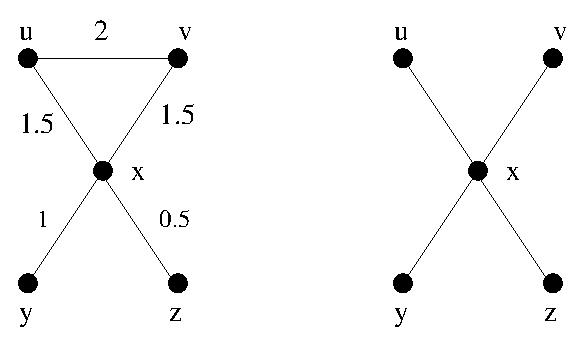
\includegraphics[scale=0.45]{figuras/exemplo_Y_minimal}
\caption{Um grafo com sua respectiva árvore t-spanner ótima}
\label{fig:exemplo_Y_minimal}
\end{figure}

No corolário \ref{corol:Yuv_define_caminho}, para $e = uv \in E(G)$, 
para mostrar que $G[F(e)]$ 
é um caminho entre $u$ e $v$, nós assumimos como hipótese que $Y'$ possui 
suporte mínimo. Esta hipótese não é condição necessária para que uma solução 
de \ref{lp:primal_mmst} seja ótima.
Considere a figura \ref{fig:exemplo_Y_minimal}. Seja $G$ o grafo do lado 
esquerdo da figura. Para $t = 2$, observe que a solução ótima de $P$ 
corresponde à árvore no lado direito (para $t = 1.5$, a árvore também é 
$t$-spanner). 
%, cujo fator de dilatação $t^*$ é $1.5$. 
Seja $H$ esta árvore. Vamos 
construir uma solução viável $(x^*,Y^*)$ para \ref{lp:primal_mmst} diferente de 
$H$. Para cada $e=pq, f \in E(G)$, defina $x^*$ e $Y^*$ da seguinte forma: 
%aplicando a construção apresentada na afirmação \ref{afirm:sol_viavel_lp}, 
% definida pelas atribuições \ref{regra:1} e 10, 
% substituindo a atribuição \ref{regra:2b} pela seguinte atribuição:

\begin{align*}
&x^*(e) \leftarrow \incid^{H}_{e},\\
&Y^*(e,f)\leftarrow
\begin{cases}
    1& \text{se $f \in E(H_{p,q}),$}\\
    1& \text{se $e = xy, f = xz,$}\\
    0& \text{se $f \in E(G) \setminus E(H_{p,q}).$}
\end{cases}
%&t^* \leftarrow \text{valor suficientemente grande que satisfaça a restrição }\ref{res_mmst:spanner} \text{ para } x^* \text{ e } Y^*.
\end{align*}
É fácil verificar que $(x^*,Y^*)$ é uma solução viável (ótima) de \ref{lp:primal_mmst} 
tal que $Y^*$ não tem suporte mínimo.

\section{Separação das Inequações de Corte}

Na formulação \ref{lp:primal_mmst}, o número de inequações correspondentes à 
restrição (\ref{res_mmst:path}), as quais são conhecidas como 
\emph{inequações de corte}, é exponencial no tamanho de $V(G)$. 
Para tratar 
as restrições de tamanho exponencial, precisamos resolver o problema da 
separação. No problema da separação, dado um conjunto de inequações e uma 
(possível) solução, nós queremos saber se existe uma inequação violada pela 
solução. 
Em outras palavras, desejamos saber se a solução é viável ou obter um 
certificado que corresponda a uma inequação violada. 
%mostra que a solução é viável ou exiba uma restrição violada.

A separação das inequações de corte de \ref{lp:primal_mmst} 
pode ser feita em tempo polinomial. Para um $t \ge 1$, seja $(x^*, Y^*)$ uma 
(possível) solução 
de \ref{lp:primal_mmst}. 
%Podemos interpretar a restrição \ref{res_mmst:path} da seguinte forma: 
Para cada $e=uv \in E(G)$, seja $G_{e} = (V, E')$, onde 
$E' = E(G)$ e $w(f) \leftarrow Y^*(e,f), \forall f \in E'$. A capacidade de 
um $(u,v)$-corte mínimo em $G_{e}$ deve ser maior ou igual a $1$. Caso 
exista 
um $e=uv \in E(G)$ tal que um $(u,v)$-corte mínimo $\delta(W)$ em $G_{e}$ 
tenha capacidade menor do que $1$, então o par $(e,W)$ é um certificado de que a 
restrição \ref{res_mmst:path} é violada. Em decorrência do 
valor de um $(u,v)$-fluxo máximo ser igual à capacidade de um 
$(u,v)$-corte mínimo \cite{DantzigF1956}, existe um algoritmo de 
separação para as inequações de corte, cuja complexidade 
computacional é $O(|E(G)|^{2} \cdot |V(G)|^{2})$ (teorema 8.30 em 
\cite{KorteV2012}).

%\section{Dimensão do Poliedro $(P(G,t))_{I}$}
\section{Facetas do Poliedro dos Grafos t-spanner}
Seja $E(G) = \{e_1, e_2, ..., e_m\}$. Seja $x \in \espacoX, Y \in \espacoY$, 
onde $Y = (Y_{e_1}^{|E(G)|}, Y_{e_2}^{|E(G)|}, ..., Y_{e_m}^{|E(G)|})$. 
Para $(x^{F'},Y^{F}) \in P(G,t)$, interpretamos os vetores da seguinte forma: 
$x^{F'}$ representa o vetor de incidência de $F' \subseteq E(G)$ em $x$; 
para $e = uv \in E(G)$, existe $P \in \PathuvF$ tal que 
$Y(e,f) = 1, \forall f \in E(P)$. 
Para $(x^{F'},(Y_{e_1}^{F_{e_1}},...,Y_{e_m}^{F_{e_m}})) \in P(G,t)$, os vetores 
$x^{F'}$ e $Y_{e_i}^{F_{e_i}}, \forall e_i \in E(G)$, representam os vetores de 
incidência de $F' \subseteq E(G)$ e $F_{e_i} \subseteq E(G)$ em $x$ e $Y_{e_i}$, 
respectivamente.

\begin{lema}
$dim((P(G,t))_{I}) = |E(G)|(|E(G)|+1) - (|\Bridge|+\sum_{uv \in E(G)}|\Bridgeuv|)$.

\begin{proof}
Seja $f \in \Bridge$. Seja $(x',Y') \in (P(G,t))_I$. 
Seja $e'=u'v' \in E(G)$ tal que $\BridgeuvPrime \neq \emptyset$. Seja 
$f'\in \BridgeuvPrime$. Então $Y'(e',f') = 1$ e $x'(f') = 1$.
Logo, \\
\mbox{$dim((P(G,t))_{I}) \le |E(G)|(|E(G)|+1) - (|\Bridge|+\sum_{uv \in E(G)}|\Bridgeuv|)$}.

Seja $e_i=uv \in E(G), f \in E(G) \setminus \Bridgeuv$. Então \\
\mbox{$(x^{E(G)}, (Y_{e_1}^{E(G)}, ..., Y_{e_i}^{E(G)-f}, ..., Y_{e_m}^{E(G)})) \in (P(G,t))_{I}$}. Seja $f' \in E(G) \setminus \Bridge$. Então 
$(x^{E(G)-f'},(Y_{e_1}^{E(G)-f'},...,Y_{e_m}^{E(G)-f'})) \in (P(G,t))_{I}$.
%$(x^{E(G)-f'}, (Y_{e_1}^{E(G)-f'}, ..., Y_{e_m}^{E(G)-f})) \in (P(G,t))_{I}$. 
Note também que \\
\mbox{$(x^{E(G)},(Y_{e_1}^{E(G)},...,Y_{e_m}^{E(G)})) \in (P(G,t))_{I}$}. 
Observe que estes vetores formam um conjunto afim independente. Segue que \\
\mbox{$dim((P(G,t))_{I}) \ge |E(G)|(|E(G)|+1) - (|\Bridge|+\sum_{uv \in E(G)}|\Bridgeuv|)$}, concluindo a prova.
\end{proof}
\end{lema}

Ao longo desta seção provaremos que algumas inequações de $P(G,t)$ definem 
e outras não definem 
facetas. Alguns resultados são baseados no trabalho de Aneja \cite{Aneja1980}.
% Também mostraremos que a inequação definida pela restrição \ref{res_mmst:spanner} 
% não define faceta de $P(G,t)$.
%definidas pela relaxação linear do PL \ref{lp:primal_mmst} definem facetas. 
%Assuma que o grafo $G$ é $t$-spanner.
% Vamos provar que a inequação definida pela restrição \ref{res_mmst:path} 
% define uma faceta. Para isso, necessitamos de uma definição. Assuma que 
% $G$ seja um grafo $t$-spanner. Uma aresta $e \in E(G)$ é uma 
% \emph{ponte t-spanner} se e somente se $G - e$ não é um grafo $t$-spanner. 

\begin{lema}
\label{lem:x_not_facet}
Seja $f \in E(G) \setminus \Bridge$. A inequação $x(f) \ge 0$ 
não define faceta de $(P(G,t))_I$.
\begin{proof}
Seja $\facetF_f = \{(x^{F},Y^{F}) \in (P(G,t))_I\; |\; x(f) = 1\}$. Seja 
$(x',Y') \in \facetF_f$. 
Seja $e'=uv \in E(G)$ tal que $\BridgeuvPrime \neq \emptyset$. Seja 
$f'\in \BridgeuvPrime$. Então $Y'(e',f') = 1$ e $x'(f') = 1$. 
Ademais, $x'(f) = 0$. Em decorrência da restrição 
\ref{res_mmst:relate_vars} de $P(G,t)$, segue que 
$Y'(e,f) = 0, \forall e \in E(G)$. Podemos concluir que \\
\mbox{$dim(\facetF_f) \le |E(G)|(|E(G)|+1) - (|B(t,G)|+\sum_{uv \in E(G)}|\Bridgeuv|) - 1 - |E(G)|$.}
\end{proof}
\end{lema}

% \begin{lema}
% Seja $f \in E(G) \setminus B(t,G)$. A inequação $x(f) \ge 0$ define faceta de 
% $P(G,t)$ se e somente se $B(t,G-f,G) = B(t,G)$.
% \begin{proof}
% $(\Leftarrow)$ Seja $F_f = \{(\incid^{F},\incidY^{F}) \in P(G,t)\; |\; x(f) = 0\}$. 
% Seja $g \in E(G) \setminus B(t,G), g \neq f$. 
% Como $f \in E(G) \setminus B(t,G)$ e $B(t,G-f,G) = B(t,G)$, então 
% $(\incid^{E(G)-f},\incidY^{E(G)-f}), (\incid^{E(G)-f-g},\incidY^{E(G)-f-g}) \in P(G,t)$. 
% Ademais, $(\incid^{E(G)-f},\incidY^{E(G)-f})$,\\ 
% $(\incid^{E(G)-f-g},\incidY^{E(G)-f-g}) \in F_f$. 
% Além disso, $(\incid^{E-f},\incidY^{E-f})$ e 
% $(\incid^{E(G)-f-g},\incidY^{E(G)-f-g})$, 
% $\forall g \in E(G) \setminus B(t,G)$ e $g \ne f$, 
% são afim independentes.

% $(\Rightarrow)$ Suponha (por absurdo) que $\exists g \in E(G) \setminus B(t,G)$ tal que 
% $g \in B(t,G-f,G)$. % seja ponte $t$-spanner de $G-f$. 
% Então a inequação $x(f) + x(g) \ge 1$ é válida para 
% $P(G,t)$. %pois $g \notin B(t,G)$. %não é ponte $t$-spanner de $G$. 
% Além disso, sabemos que 
% a inequação $-x(g) \ge -1$ é válida para $P(G,t)$. Mas então, a inequação 
% $x(f) \ge 0$ pode ser obtida através da soma destas duas inequações anteriores, 
% contradizendo o fato de que $x(f) \ge 0$ define faceta.
% \end{proof}
% \end{lema}

\begin{lema}
Seja $e = uv \in E(G)$. 
Seja $f \in E(G) \setminus \Bridge$ tal que 
$\BridgeuvGf = \BridgeuvPrimeGf, \forall (u',v') \in \BridgeTwoGf$. %e $(u'v') \neq (u,v)$. 
A inequação $Y(e,f) \ge 0$ define faceta de 
$(P(G,t))_{I}$ se e somente se $\BridgeGf = \Bridge$.
\begin{proof}
$(\Leftarrow)$ Seja $\facetF_f = \{(x^{F},Y^{F}) \in (P(G,t))_I\; |\; Y(e,f) = 0\}$. 
Seja $g \in E(G) \setminus \Bridge, g \neq f$. 
Seja $e = e_i$. Considere estes três conjuntos de vetores pertencentes a $(P(G,t))_{I}$:
\begin{itemize}
  \item $(x^{E(G)},(Y_{e_1}^{E(G)}, ..., Y_{e_i}^{E(G)-f-g}, ..., Y_{e_m}^{E(G)})) \in (P(G,t))_{I}$, visto que \\
\mbox{$f \in E(G) \setminus \Bridge$ e $\BridgeGf = \Bridge$};
  \item $(x^{E(G)},(Y_{e_1}^{E(G)}, ..., Y_{e_j}^{E(G)-g}, ..., Y_{e_i}^{E(G)-f}, ..., Y_{e_m}^{E(G)})) \in (P(G,t))_{I}$, \\$\forall e_j \in E(G), e_j \neq e_i$, visto que 
$g \in E(G) \setminus \Bridge$;
  \item $(x^{E(G)-g},(Y_{e_1}^{E(G)-g}, ..., Y_{e_i}^{E(G)-f-g}, ..., Y_{e_m}^{E(G)-g})) \in (P(G,t))_{I}$, visto que \\
\mbox{$f \in E(G) \setminus \Bridge$ e $\BridgeGf = \Bridge$}.
\end{itemize} 
%$(\incid^{E(G)-f},\incidY^{E(G)-f}), (\incid^{E(G)-f-g},\incidY^{E(G)-f-g}) \in P(G,t)$. 
Ademais, a coleção acima de vetores pertence a $\facetF_f$. Além disso, estes vetores 
são afim independentes.%\\
% $(\incid^{E(G)-f},\incidY^{E(G)-f})$, 
% $(\incid^{E(G)-f-g},\incidY^{E(G)-f-g}) \in F_f$. 
% Além disso, $(\incid^{E(G)-f},\incidY^{E(G)-f})$ e 
% $(\incid^{E(G)-f-g},\incidY^{E(G)-f-g})$, $\forall g \in E(G) \setminus B(t,G)$ e $g \ne f$, 
% são afim independentes.

$(\Rightarrow)$ Suponha (por absurdo) que $\exists g \in E(G) \setminus \Bridge$ tal que 
$g \in \BridgeGf$. %$t$-spanner de $G-f$. 
Como $\BridgeuvGf = \BridgeuvPrimeGf, \forall (u',v') \in \BridgeTwoGf$, 
então a inequação $Y(e,f) + Y(e,g) \ge 1$ é válida para 
$P(G,t)$ pois %$g \notin B(t,G)$ e 
$g \in \BridgeuvGf$. %não é $(u,v,t,G)$-ponte. 
Além disso, sabemos que 
a inequação $-Y(e,g) \ge -1$ é válida para $P(G,t)$. Mas então, a inequação 
$Y(e,f) \ge 0$ pode ser obtida através da soma destas duas inequações anteriores, 
contradizendo o fato de que $Y(e,f) \ge 0$ define faceta.
\end{proof}
\end{lema}

\begin{lema}
Seja $f \in E(G) \setminus \Bridge$. A inequação $x(f) \le 1$ define faceta de 
$(P(G,t))_{I}$.
\begin{proof}
Seja $\facetF_f = \{(x^{F},Y^{F}) \in (P(G,t))_I\; |\; x(f) = 1\}$. 
Considere estes dois conjuntos de vetores pertencentes a $(P(G,t))_{I}$:
\begin{itemize}
  \item $(x^{E(G)}, (Y_{e_1}^{E(G)},...,Y_{e_i}^{E(G)-g'},...,Y_{e_m}^{E(G)})) \in (P(G,t))_I$,
 \\
$\forall e_i \in E(G), \forall g' \in E(G) \setminus \Bridge$;
  \item $(x^{E(G)-g}, Y^{E(G)-g}) \in (P(G,t))_I$, 
$\forall g \in E(G) \setminus \Bridge, g \neq f$. 
\end{itemize}
% Seja $g \in E(G) \setminus B(t,G), g \neq f$. 
% Como $g \in E(G) \setminus B(t,G)$, $(\incid^{E(G)},\incidY^{E(G)}), (\incid^{E(G)-g},\incidY^{E(G)-g}) \in P(G,t)$. 
Ademais, a coleção acima de vetores pertence a $\facetF_f$. 
Além disso, estes vetores são afim independentes.
\end{proof}
\end{lema}

\begin{lema}
\label{lem:Y_not_facet}
Seja $e \in E(G), f \in E(G) \setminus \Bridge$. A inequação $Y(e,f) \le 1$ 
não define faceta de $(P(G,t))_I$.
\begin{proof}
Seja $\facetF_f = \{(x^{F},Y^{F}) \in (P(G,t))_I\; |\; Y(e,f) = 1\}$. Seja 
$(x',Y') \in \facetF_f$. Seja $e'=u'v' \in E(G)$ tal que 
$\BridgeuvPrime \neq \emptyset$. Seja 
$f'\in \BridgeuvPrime$. 
Então $Y'(e',f') = 1$ e $x'(f') = 1$. Ademais, 
$Y'(e,f) = 1$. Em decorrência da restrição \ref{res_mmst:relate_vars} de 
$P(G,t)$, segue que $x'(f) = 1$. Podemos concluir que \\
\mbox{$dim(\facetF_f) \le |E(G)|(|E(G)|+1) - (|\Bridge|+\sum_{uv \in E(G)}|\Bridgeuv|) - 2$.}
\end{proof}
\end{lema}

\begin{lema}
Seja $e \in E(G), f \in E(G) \setminus \Bridge$. A inequação $Y(e,f) \le x(f)$ 
não define faceta de $(P(G,t))_{I}$.
\begin{proof}
Seja $\facetF_f = \{(x^{F},Y^{F}) \in (P(G,t))_I\; |\; Y(e,f) = x(f)\}$. 
Para $x(f) = 0$, segue do lema \ref{lem:x_not_facet}. 
Para $Y(e,f) = 1$, segue do lema \ref{lem:Y_not_facet}. 
Para $Y(e,f) = 0$ e $x(f) = 1$, segue que 
\mbox{$dim(\facetF_f) \le |E(G)|(|E(G)|+1) - (|\Bridge|+\sum_{uv \in E(G)}|\Bridgeuv|) - 2$}, concluindo a prova.
\end{proof}
\end{lema}

% \begin{lema} 
% Sejam $e=uv \in E(G)$ e $f \in E(G) \setminus B(t,G)$ tal que para cada 
% $(u,v,t,G)$-caminho $P_{u,v}, \dist_{P_{u,v}}(u,v) + c(f) > t \cdot dist_{G}(u,v)$. 
% A inequação $Y(e,f) \le 1$ define faceta de $P(G,t)$ se e somente se existe 
% um $(u,v,t,G)$-caminho $P$ tal que $f \in E(P)$.
% \begin{proof}
% $(\Leftarrow)$
% Seja $F_{f} = \{(\incid^{F},\incidY^{F}) \in P(G,t)\; |\; Y(e,f) = 1\}$. 
% Seja $g \in E(G) \setminus B(t,G), g \neq f$. 
% Como 
% $g \in E(G) \setminus B(t,G)$, então 
% $(\incid^{E(G)},\incidY^{E(G)})$, $(\incid^{E(G)-g}$, $\incidY^{E(G)-g}) \in P(G,t)$. 
% Por hipótese, $P$ é um $(u,v,t,G)$-caminho. Então, vamos assumir que 
% $Y(e,h) = 1, \forall h \in E(P)$. Note que $f \in E(P)$. 
% Então, $(\incid^{E(G)},\incidY^{E(G)})$, \\
% $(\incid^{E(G)-g},\incid^{E(G)-g}) \in F_f$. 
% Ademais, $(\incid^{E(G)},\incidY^{E(G)})$ e 
% $(\incid^{E(G)-g},\incidY^{E(G)-g}), \forall g \in E(G) \setminus B(t,G)$  $g \neq f$, 
% são afim independentes.

% $(\Rightarrow)$
% Suponha (por absurdo) que para cada $(u,v,t,G)$-caminho $P$, $f \notin E(P)$. 
% Como $Y(e,f) \le 1$ define faceta, $\exists (\incid^{F},\incidY^{F}) \in P(G,t)$ 
% tal que $Y(e,f) = 1$. Seja $P \subseteq G[F]$ um $(u,v,t,G)$-caminho tal que 
% $Y(e,g) = 1, \forall g \in E(P)$ (proposição \ref{prop:Yuv_caminho}). 
% Como $f \notin E(P)$, então 
% \begin{align*}
% \sum_{g \in E(G)}Y(e,g) &= \sum_{g \in F}Y(e,g)\\ 
% &\ge \sum_{h \in E(P)}(Y,h) + Y(e,f)\\
% &> t \cdot dist_{G}(u,v),
% \end{align*}
% onde a igualdade decorre da restrição \ref{res_mmst:relate_vars}. Logo, a relação 
% acima contradiz o fato de $(\incid^{F},\incidY^{F}) \in P(G,t)$ (viola a restrição 
% \ref{res_mmst:spanner}).
% \end{proof}
% \end{lema}

% \begin{lema}
% Seja $e = uv \in E(G)$. A inequação

% \begin{equation*}
% \label{fac_spanner}
% \sum_{f \in E(G)}Y(e,f) w(f) \le t \cdot \dist_{G}(u,v)
% \end{equation*}
% não define uma faceta de $P(G,t)$.
% \begin{proof}
% Suponha (por absurdo), que esta inequação defina faceta. 
% Seja $F_W = \{(\incid^{F},\incidY^{F})\; |\; \sum_{f \in E(G)}Y(e,f)w(f) = t \cdot dist_{G}(u,v)\}$. 
% Seja $(\incid^{F},\incidY^{F}) \in F_W$ (por suposição, $F_W \neq \emptyset$). 
% Seja $F(e) = \{f \in F\; |\; Y(e,f) = 1\}$. Note que $\forall f \in F(e)$,

% \begin{align*}
% Y(e,f)w(f) &\le x(f)w(f)\\
% x(f)w(f) &\le w(f),
% \end{align*}
% onde a primeira inequação decorre da restrição \ref{res_mmst:relate_vars} e a 
% segunda decorre da restrição \ref{res_mmst:int_x}. Sendo assim, a seguinte 
% inequação é válida: 

% \begin{equation*}
% \sum_{f \in F(e)}Y(e,f)w(f) \le t \cdot dist_{G}(u,v).
% \end{equation*}

% Ademais, como $(\incid^{F},\incidY^{F}) \in P(G,t)$ (ou seja, deve respeitar a 
% restrição \ref{res_mmst:spanner}) e 
% $(\incid^{F},\incidY^{F}) \in F_W$ (ou seja, a restrição \ref{res_mmst:spanner} 
% é respeitada com igualdade), então 
% $Y(e,f) \le 0, \forall f \in E(G) \setminus F(e)$. Logo, a seguinte inequação 
% é válida:

% \begin{equation*}
% \sum_{f \in E(G) \setminus F(e)}Y(e,f)w(f) \le 0.
% \end{equation*}

% A soma destas duas inequações válidas resulta na inequação 
% $\sum_{f \in E(G)}Y(e,f) w(f) \le t \cdot \dist_{G}(u,v)$, contradizendo o fato 
% dela definir faceta.
% \end{proof}
% \end{lema}

\begin{teorema}
Seja $e = uv \in E(G)$. Seja $\delta(W)$ um $(u,v)$-corte, 
onde $\overline{W} = V(G) \setminus W$, com as seguintes propriedades: %tal que

\begin{enumerate}
\item \label{fac_corte:cam_W}
Para cada $p,q \in W$, existe um caminho em $\PathpqW$ (a propriedade vale 
substituindo $W$ por $\overline{W}$);

\item \label{fac_corte:ponte_W}
Para cada $p,q \in W$ e para cada $g \in E(W) \cup E(\overline{W})$, existe um caminho em $\PathpqWg$ (a propriedade vale substituindo $W$ por 
$\overline{W}$).
\end{enumerate}

A inequação

\begin{equation*}
%\label{fac_corte:inequacao}
Y(e, \delta(W)) \ge 1
\end{equation*}
define uma faceta de $(P(G,t))_{I}$ se e somente se:

\begin{enumerate}
% \item \label{fac_corte:cam_W}
% Para cada $p,q \in W$, existe um $(p,q,t,G[W],G)$-caminho;

% \item \label{fac_corte:ponte_W}
% Para cada $p,q \in W$ e para cada $g \in E(W) \cup E(\overline{W})$, existe um 
% $\mbox{(p,q,t,G[W]-g,G)}$-caminho.

\item \label{fac_corte:cam_W_Wbar}
Para cada $p \in W, q \in \overline{W}$ e para cada 
$f \in \delta(W)$, existe um caminho em $\PathpqWWbarf$ (a condição vale 
substituindo $W$ por $\overline{W}$). 

\item \label{fac_corte:ponte_W_Wbar}
Para cada $p \in W,q \in \overline{W}$, para cada $f \in \delta(W)$ 
e para cada $g \in E(W)$, existe um caminho em $\PathpqWWbarfg$ (a condição vale substituindo 
$g \in E(W)$ por $g \in E(\overline{W})$). 
\end{enumerate}

% \emph{Na condição (\ref{fac_corte:cam_W}),
% podemos substituir $W$ por $\overline{W}$. 
% Na condição  (\ref{fac_corte:ponte_W_Wbar}), 
% podemos substituir $g \in E(W)$ por $g \in E(\overline{W})$}.

\begin{proof}
Seja 
\begin{equation*}
\begin{split}
\facetF_{W} = \{(x^{F},Y^{F}) \in P(G,t)\; |\; Y(e,\delta(W)) = 1\} \subseteq \\ 
\{(x^{F},Y^{F}) \in P(G,t)\; |\; &\alpha \cdot (\sum_{f \in E(G)}Y(e,f)) + \\
 &\beta \cdot (\sum_{e' \in E(G) - e, f \in E(G)}Y(e',f)) +\\
 &\gamma \cdot (\sum_{e" \in E(G)}x(e")) = \theta\} = \facetF.
\end{split}
\end{equation*}

% $(\Leftarrow)$ Vamos provar a suficiência mostrando que qualquer outra inequação válida 
% tal que a inclusão acima valha, é múltiplo não negativo de $Y(e,\delta(W)) \ge 1$. 
% Seja $f \in \delta(W)$. Seja $B \leftarrow E(W) \cup E(\overline{W})$. 
% Como valem a propriedade (\ref{fac_corte:cam_W}) e a hipótese 
% (\ref{fac_corte:cam_W_Wbar}), então $(\incid^{B+f},\incidY^{B+f}) \in F_{W}$. 
% Como valem a propriedade (\ref{fac_corte:ponte_W}) e a hipótese 
% (\ref{fac_corte:ponte_W_Wbar}), 
% segue que $(\incid^{B+f-g},\incidY^{B+f-g}) \in F_{W}$. 

% Vamos assumir que tanto para $(\incid^{B+f},\incidY^{B+f})$ como para 
% $(\incid^{B+f-g},\incidY^{B+f-g})$, $Y$ tem suporte mínimo (podemos assumir isso 
% em decorrência do corolário \ref{corol:Y_suporte_minimo}).

% Como $(\incid^{B+f},\incidY^{B+f}), (\incid^{B+f-g},\incidY^{B+f-g}) \in F$, então 
% $\alpha \cdot (\sum_{h \in B}Y(e,h) + Y(e,f)) = \beta = \alpha \cdot (\sum_{h \in B-g}Y(e,h) + Y(e,f))$. 
% Isto implica que $\alpha_{g} = 0, \forall g \in E(W) \cup E(\overline{W})$.

% Seja $f,g \in \delta(W), f \neq g$. Como valem a propriedade (\ref{fac_corte:cam_W}) 
% e a hipótese (\ref{fac_corte:cam_W_Wbar}), então 
% $(\incid^{B+f},\incidY^{B+f}), (\incid^{B+g},\incidY^{B+g}) \in F_W$ e, por 
% consequência, pertencem a $F$. Sendo assim, 
% $\alpha \cdot (\sum_{h \in B}Y(e,h) + Y(e,f)) = \beta = \alpha \cdot (\sum_{h \in B}Y(e,h) + Y(e,g))$. 
% Então, $\alpha_{f} = \alpha_{g} = \beta, \forall f,g \in \delta(W)$.

% Logo,
% \begin{align*}
% &\alpha_{i}\leftarrow
% \begin{cases}
%     \beta,& \text{se $i \in \delta(W)$},\\
%     0,& \text{caso contrário},
% \end{cases}
% \end{align*}
% provando que $Y(e, \delta(W)) \ge 1$ define uma faceta de $P(G,t)$ quando as 
% propriedades no enunciado são satisfeitas.

$(\Leftarrow)$ Vamos provar a suficiência mostrando que qualquer outra inequação 
válida $\alpha \cdot (\sum_{f \in E(G)}Y(e,f)) + \beta \cdot (\sum_{e' \in E(G) - e, f \in E(G)}Y(e',f)) + \gamma \cdot (\sum_{e" \in E(G)}x(e")) \ge \theta$
tal que a inclusão acima valha, é múltiplo não negativo de $Y(e,\delta(W)) \ge 1$. 
Seja $f \in \delta(W)$. Seja $B \leftarrow E(W) \cup E(\overline{W})$. 
Como valem a propriedade (\ref{fac_corte:cam_W}) e a hipótese 
(\ref{fac_corte:cam_W_Wbar}), então 
$(x^{B+f},Y^{B+f}) \in \facetF_{W}$. 

Seja $g \in E(W) \cup E(\overline{W})$. 
Como valem a propriedade (\ref{fac_corte:ponte_W}) e a hipótese 
(\ref{fac_corte:ponte_W_Wbar}), 
segue que $(x^{B+f-g},Y^{B+f-g}) \in \facetF_{W}$. 

Como $(x^{B+f},Y^{B+f}), (x^{B+f-g},Y^{B+f-g}) \in \facetF$, então 

\begin{equation*}
\begin{split}
&\alpha \cdot ((\sum_{h \in B} Y(e,h)) + Y(e,f)) + \\
&\beta \cdot ((\sum_{e' \in E(G) - e, h \in B} Y(e',h)) + \sum_{e' \in E(G) - e}Y(e',f)) + \\
&\gamma \cdot ((\sum_{e" \in B} x(e")) + x(f)) = \theta = \\
&\alpha \cdot ((\sum_{h \in B-g} Y(e,h)) + Y(e,f)) + \\
&\beta \cdot ((\sum_{e' \in E(G) - e, h \in B-g} Y(e',h)) + \sum_{e' \in E(G) - e}Y(e',f)) + \\
&\gamma \cdot ((\sum_{e" \in B-g} x(e")) + x(f)).
\end{split}
\end{equation*}
% $\alpha \cdot (\sum_{h \in B}Y(e,h) + Y(e,f)) = \beta = \alpha \cdot (\sum_{h \in B-g}Y(e,h) + Y(e,f))$. 

Isto implica que 

%\begin{equation}
\begin{align}
\alpha_{g} &= 0, \forall g \in E(W) \cup E(\overline{W});\label{coef1}\\
\beta_{e',g} &= 0, \forall e' \in E(G)-e, \forall g \in E(W) \cup E(\overline{W});\label{coef2}\\
\gamma_{g} &= 0, \forall g \in E(W) \cup E(\overline{W})\label{coef3}.
\end{align}
%\end{equation}
Note que $\alpha_{g}$ tem que ser igual a $0, \forall g \in E(W) \cup E(\overline{W})$, 
pois nada impede que para $(x^{B+f-g},Y^{B+f-g}), Y(e,g) = 1$. De maneira 
análoga, $\beta_{e',g}$ tem que ser igual a 
$0, \forall e' \in E(G) - e, \forall g \in E(W) \cup E(\overline{W})$. 

% Observe que tanto para $(\incid^{B+f},\incidY^{B+f})$ como para 
% $(\incid^{B+f-g},\incidY^{B+f-g})$, temos que $x(f') = 0$ e 
% $Y(e',f') = 0, \forall e' \in E(G) - e, \forall f' \in \delta(W), f' \neq f$. 

% Observe também que tanto para $(\incid^{B+f},\incidY^{B+f})$ como para 
% $(\incid^{B+f-g},\incidY^{B+f-g})$, temos que $x(f) = 1$, pois $Y(e,f) = 1$ e vale a 
% restrição \ref{res_mmst:relate_vars}. 
% Ou seja, $\forall (\incid^{F},\incidY^{F}) \in F_W$ tal que $f \in F$, segue $x(f) = 1$.

% Note que tanto para $(\incid^{B+f},\incidY^{B+f})$ como para 
% $(\incid^{B+f-g},\incidY^{B+f-g})$, o valor de $\beta_{e',f}, \forall e' \in E(G) - e$, 
% é dividido em dois casos: 
% \begin{enumerate}
% \item $e' \in \delta(W)$: 
% temos que $Y(e',f) = 1$ pois $x(f) = 1$ e 
% $\forall (\incid^{F},\incidY^{F}) \in F_W, |F \cap \delta(W)| = 1$, além da 
% restrição \ref{res_mmst:path} ser respeitada. 
% Ou seja, $\forall (\incid^{F},\incidY^{F}) \in F_W$ tal que $f \in F$, segue 
% $Y(e',f) = 1$.

% \item Sem perda de generalidade, $e' \in E(W)$: como 
% $\forall (\incid^{F},\incidY^{F}) \in F_W, |F \cap \delta(W)| = 1$, além de valer a 
% propriedade \ref{fac_corte:ponte_W} e $Y$ ter suporte mínimo, então $Y(e',f) = 0$. 
% \end{enumerate}

Seja $f,g \in \delta(W), f \neq g$. Como valem a propriedade (\ref{fac_corte:cam_W}) 
e a hipótese (\ref{fac_corte:cam_W_Wbar}), então 
$(x^{B+f},Y^{B+f}), (x^{B+g},Y^{B+g}) \in \facetF_W$. 
Vamos assumir que tanto para $(x^{B+f},Y^{B+f})$ como para 
$(x^{B+g},Y^{B+g})$, $Y$ tem suporte mínimo (podemos assumir isso 
em decorrência do corolário \ref{corol:Y_suporte_minimo}). 
Observe que 
$(x^{B+f},Y^{B+f}), (^{B+g},Y^{B+g}) \in \facetF$. 
Sendo assim, 

\begin{equation*}
\begin{split}
&\alpha \cdot ((\sum_{h \in B} Y(e,h)) + Y(e,f)) + \\
&\beta \cdot ((\sum_{e' \in E(G) - e, h \in B} Y(e',h)) + \sum_{e' \in E(G) - e}Y(e',f)) + \\
&\gamma \cdot ((\sum_{e" \in B} x(e")) + x(f)) = \theta = \\
&\alpha \cdot ((\sum_{h \in B} Y(e,h)) + Y(e,g)) + \\
&\beta \cdot ((\sum_{e' \in E(G) - e, h \in B} Y(e',h)) + \sum_{e' \in E(G) - e}Y(e',g)) + \\
&\gamma \cdot ((\sum_{e" \in B} x(e")) + x(g)).
\end{split}
\end{equation*}

Então, em decorrência de (\ref{coef1}), (\ref{coef2}) e (\ref{coef3}), temos que 

\begin{equation*}
\begin{split}
&\alpha \cdot Y(e,f) + \\
&\beta \cdot ((\sum_{e' \in \delta(W) - e} Y(e',f)) + \beta \cdot (\sum_{e' \in E(W) \cup E(\overline{W})}Y(e',f)) + \\
&\gamma \cdot x(f) = \theta = \\
&\alpha \cdot Y(e,g) + \\
&\beta \cdot ((\sum_{e' \in \delta(W) - e} Y(e',g)) + \beta \cdot (\sum_{e' \in E(W) \cup E(\overline{W})}Y(e',g)) + \\
&\gamma \cdot x(g).
\end{split}
\end{equation*}

Isto implica que

\begin{equation*}
\begin{split}
\alpha_{f} &= \alpha_{g}, \forall f,g \in \delta(W);\\
\beta_{e',f} &= \beta_{e',g}, \forall e' \in E(G)-e, \forall f,g \in \delta(W);\\
\gamma_{f} &= \gamma_{g}, \forall f,g \in \delta(W).
\end{split}
\end{equation*}


Observe que para $(x^{B+f},Y^{B+f})$ 
%como para $(\incid^{B+g},\incidY^{B+g})$, 
temos que $x(f) = 1$, pois $Y(e,f) = 1$ e vale a 
restrição \ref{res_mmst:relate_vars} de $P(G,t)$. 
Ou seja, $\forall (x^{F},Y^{F}) \in \facetF_W$ tal que $f \in F$, 
segue $x(f) = 1$. Sendo assim, o coeficiente de $x(f)$ na equação que defina 
$\facetF_{W}$ é $0$.
 De maneira análoga, para $(x^{B+g},Y^{B+g})$ temos que $x(g) = 1$ e 
seu coeficiente na equação que define $\facetF_{W}$ é $0$.

Observe também que para $(x^{B+f},Y^{B+f})$ 
temos que $Y(e',f) = 1, \forall e' \in \delta(W) - e$, pois $x(f) = 1$ e 
$|F \cap \delta(W)| = 1, \forall (x^{F},Y^{F}) \in \facetF_W$, 
além da restrição \ref{res_mmst:path} ser respeitada. 
Ou seja, $\forall (x^{F},Y^{F}) \in \facetF_W$ tal que $f \in F$, 
segue que $Y(e',f) = 1, \forall e' \in \delta(W) - e$. 
De maneira análoga, para $(x^{B+g},Y^{B+g})$ 
temos que $Y(e',g) = 1, \forall e' \in \delta(W) - e$. Como argumentamos 
anteriormente, os respectivos coeficientes na equação que define $\facetF_{W}$ 
possuem valor $0$.

Para $(x^{B+f},Y^{B+f})$ temos que $Y$ tem suporte mínimo. 
Além disso, $|F \cap \delta(W)| = 1, \forall (x^{F},Y^{F}) \in \facetF_W$, e 
vale a restrição \ref{fac_corte:cam_W}. Então, segue que 
$Y(e',f) = 0, \forall e' \in E(W) \cup E(\overline{W})$. De maneira análoga, 
para $(x^{B+g},Y^{B+g})$ 
temos que $Y(e',g) = 0, \forall e' \in E(W) \cup E(\overline{W})$. 
Isto significa que $\beta_{e',f}$ e $\beta_{e',g}$ podem ter qualquer valor 
($0$, por exemplo). De qualquer forma, os termos $Y(e',f)$ e $Y(e',g)$ são 
nulos em $\facetF$.

% como $\forall (\incid^{F},\incidY^{F}) \in F_W, |F \cap \delta(W)| = 1$, 
% além de valer a propriedade \ref{fac_corte:ponte_W} e $Y$ ter suporte mínimo, então, 
% para $(\incid^{B+f},\incidY^{B+f})$, temos 
% $Y(e',f) = 0, \forall e' \in E(W) \cup E(\overline{W})$. De maneira análoga, 
% para $(\incid^{B+g},\incidY^{B+g})$, 
% temos $Y(e',g) = 0, \forall e' \in E(W) \cup E(\overline{W})$. 
% Isto significa que $\beta_{e',f}$ e $\beta_{e',g}$ podem ter qualquer valor 
% ($0$, por exemplo).

Logo,
\begin{align*}
&\alpha_{i}\leftarrow
\begin{cases}
    \theta,& \text{se $i \in \delta(W)$},\\
    0,& \text{caso contrário},
\end{cases}\\
&\beta_{i,j}\leftarrow 0, \forall i \in E(G)-e, j \in E(G),\\
&\gamma_{i}\leftarrow 0, \forall i \in E(G),
% &\gamma_{i}\leftarrow
% \begin{cases}
%     \frac{\theta}{|\delta(W)|+1},& \text{se $i \in \delta(W)$},\\
%     0,& \text{caso contrário},
% \end{cases}
\end{align*}
provando que $Y(e, \delta(W)) \ge 1$ define uma faceta de $(P(G,t))_{I}$ quando as 
propriedades no enunciado são satisfeitas.

Vamos agora provar a necessidade. Por hipótese, vamos assumir que 
$Y(e,\delta(W)) \ge 1$ define faceta (quando as propriedades \ref{fac_corte:cam_W} 
e \ref{fac_corte:ponte_W} são satisfeitas), ou seja, $\facetF_{W} \neq \emptyset$.

% (\ref{fac_corte:cam_W}) $\Rightarrow$ Seja $(\incid^{F},\incidY^{F}) \in F_{W}$. 
% Suponha (por absurdo) que $\exists p,q \in W$ tal que 
% $\not \exists (p,q,t,G[W],G)$-caminho. Como $Y(e,\delta(W)) \ge 1$ define 
% faceta, podemos assumir 
% que $G[F]$ é $t$-spanner, ou seja, existe um $(p,q,t,G[F],G)$-caminho. Como 
% $|\delta_{F}(W)| = 1$ e o custo das arestas é não negativo, 
% $\exists (p,q,t,G[S_{W}],G)$-caminho, onde 
% $F_{W} \subset F, F_{W} \subseteq E(W)$, uma contradição.

% (\ref{fac_corte:ponte_W}) $\Rightarrow$ Suponha (por absurdo) que 
% $\exists p, q \in W$ tal que $\exists g \in E(W)$ tal que $\not \exists$ um 
% $(p,q,t,G[W]-g,G)$-caminho. 
% Vamos mostrar que toda solução $(\incid^{F},\incidY^{F}) \in F_{W}$ contém $g$. Se a 
% inequação $x(g) \ge 1$ é válida para $P(G,t)$ e 
% $F_{W} \subseteq \{(\incid^{F},\incidY^{F}) \in P(G,t)\; |\; x(g) = 1\}$, mas 
% como $x(g) \ge 1$ não é múltiplo de $Y(e,\delta(W)) \ge 1$, então $Y(e,\delta(W) \ge 1$ 
% não define faceta.

% Suponha que $\exists (\incid^{F},\incidY^{F}) \in F_{W}$ tal que $g \notin F$. 
% Não precisamos considerar o caso em que $g \in E(\overline{W})$. 
% Sabemos que $\exists (p,q,t,G[W],G)$-caminho (hipótese \ref{fac_corte:cam_W}). 
% Como $\not \exists (p,q,t,G[W]-g,G)$-caminho, então deve existir um 
% $(p,q,t,G[S-g])$-caminho que passa por duas arestas de $\delta(W)$. Mas isto 
% contradiz o fato de $(\incid^{F},\incidY^{F})$ pertencer a $F_{W}$.

% Logo, $g \in S \forall (\incid^{S},\incidY^{S}) \in F_{W}$, contradizendo o fato 
% de $Y(e,\delta(W) \ge 1$ definir faceta.

(\ref{fac_corte:cam_W_Wbar}) $\Rightarrow$ Suponha (por absurdo) que 
$\exists p \in W, q \in \overline{W}$ tal que $\exists f \in \delta(W)$ tal que 
$\not \exists$ um caminho em $\PathpqWWbarf$. 
Seja $g=xy \in \delta(W)$ tal que $(x^{F},Y^{F}) \in \facetF_{W}$ e $g \in F$. 
Observe que $g \neq f$. Sem perda de generalidade, 
assuma que $|W| \ge 2$ (caso contrário, se $|W| = |\overline{W}| = 1$, então $f = g$). 
Como $G[F]$ é conexo pois $G[F]$ é $t$-spanner, então 
$|E(W)| \ge 1$. Como podemos assumir que vale a propriedade \ref{fac_corte:ponte_W}, 
então $|E(W)| \ge 2$. Logo, $|W| \ge 3$. Seja $W" = \{u,x\}$, se $u \neq x$, ou 
$W" = \{u\}$, caso contrário. 
Seja $W = W' \cup W"$ e 
$W'\cap W" = \emptyset$. Observe que $Y(e,\delta(W' \cup \overline{W})) \ge 1$
 é válida, pois $\delta(W' \cup \overline{W})$ é um $(u,v)$-corte e 
$g \in \delta(W' \cup \overline{W})$. Observe também que 
$Y(e,E(W',\overline{W})) \ge 0$ é válida. Somando estas duas inequações nós 
obtemos $Y(e,\delta(W)) \ge 1$, contradizendo o fato desta última inequação definir 
faceta. 

(\ref{fac_corte:ponte_W_Wbar}) $\Rightarrow$ Suponha (por absurdo) que 
$\exists p \in W, q \in \overline{W}$ tal que $\exists f \in \delta(W)$ tal que 
$\exists g \in E(W)$ tal que $\not \exists$  um caminho em $\PathpqWWbarfg$. 
Nós vamos mostrar 
que toda solução pertencente a $\facetF_{W}$ e que contenha $f$ também contém $g$. 
Se a inequação $x(g) \ge 1$ é válida para 
$\facetF_f(G,t) = \{(x^{F},Y^{F}) \in P(G,t)\;|\;f \in F\}$ e 
$\facetF_f(G,t) \subseteq \{(x^{F},Y^{F}) \in \facetF_f(G,t)\;|\;x(g) = 1\}$, 
mas $x(g) \ge 1$ não é múltiplo de $Y(e,\delta(W)) \ge 1$, então 
$Y(e,\delta(W))$ não define faceta de $(P(G,t))_{I}$.

Sabemos que $\exists (x^{F},Y^{F}) \in \facetF_W$ tal que $f \in F$ 
(hipótese \ref{fac_corte:cam_W_Wbar}). 
Suponha que $\exists (x^{F},Y^{F}) \in \facetF_{W}$ tal que $f \in F$ e 
$g \notin F$. Mas isto contradiz a nossa hipótese inicial, concluindo a prova. 
\end{proof}
\end{teorema}

 \bibliographystyle{amsplain}

 \bibliography{mmst}

\end{document}